\section{Introduction}\label{sec:intro}

Bio-signal sensing is a cornerstone in the fields of medical diagnostics, neuroscience research, and healthcare monitoring. Accurate measurement and analysis of bio-signals such as electrocardiograms (ECG), electromyograms (EMG), electroencephalograms (EEG), local field potentials (LFP), and action potentials (AP) are paramount for the effective diagnosis and treatment of a wide range of medical conditions. Each of these bio-signals possesses distinct amplitude and frequency characteristics, as depicted in \cref{fig:application}.


\begin{figure} [!htbp]
    \centering
    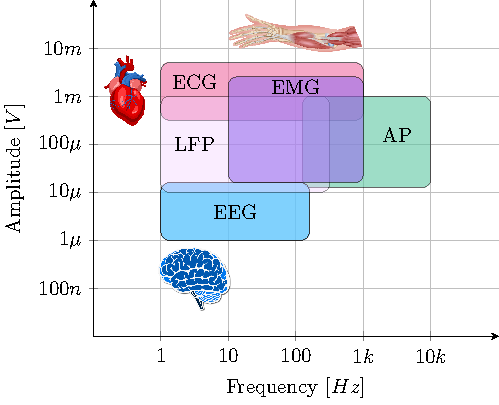
\includegraphics[ width = 0.7\columnwidth]{img/application.pdf} 
    \caption{ Typical amplitude and frequency characteristic of various bio-signals }
    \label{fig:application}
\end{figure}

 The development of low-noise analog-front-end (AFE) designs enhances the quality of bio-signal acquisition. Low-noise AFEs add minimal excess noise avoiding degradation of the signal-to-noise ratio (SNR), which is critical for obtaining clear and accurate recordings. Given that these bio-sensors may be battery-operated, power optimization becomes essential to prolong their operational life. Furthermore, sensors used in \textit{in vivo} applications must be compact to minimise invasiveness.
A chopper-stabilised capacitively coupled instrumentation amplifier (CCIA) is a versatile, low-noise amplifier topology suitable for sensor interface designs \cite{Jiang-8588386, chand-7417924}.

Designing a low-power, area-aware CCIA is a non-trivial process. Typically, designers find themselves sizing weakly/moderately inverted transistors \cite{6015500}. \gmID design \cite{jespers2017systematic} is a methodology that enables faster optimisation of the initial design, reducing the amount of SPICE simulations and time required. In the \gmID design methodology look-up tables of device properties are generated from PDK models. Toolkits consisting of data generating scripts and linear interpolating functions are used to aid the designer in visualising design trade-offs. Previous toolkits have been implemented in MATLAB \cite{MurmannGMID}. The commercial license cost of MATLAB has slowed \gmID adoption in industry. Furthermore, recent open-source circuit designs are disseminated using Jupyter Notebook (a Python-based tool) \cite{herman2024versatility} identifying a need for a \gmID package that will fit this workflow.

Here we introduce a methodology for optimising bio-sensing amplifier design using the \gmID technique. The approach enables the identification of area-aware CCIA designs while optimising noise and power consumption. The CCIA design flow is performed using PyGMID \cite{O_Donnell_PyGMID}; an enhanced, open-source python \gmID toolkit. A repeatable design flow recorded in a Jupyter Notebook \cite{CCIA_GMID} allows visualisation and insights into CCIA design optima. This paper is structured as follows: \cref{sec:background} introduces the design equations for a CCIA. A detailed CCIA design procedure is described in \cref{sec:methods}. Optimisation with an emphasis on area-aware designs suitable for \textit{in vivo} and multi sensor interfaces are discussed. \Cref{sec:implementation} describes a CCIA implemented using the \gmID design flow. \Cref{sec:results} discusses measured results for the CCIA design.